\chapter{Visualização volumétrica}
\label{cap:vis_vol}

Para a visualização volumétrica dos modelos, o InVesalius dispõe de uma técnica
conhecida como \textit{Raycasting}. Trata-se de uma técnica que,
resumidamente, consiste em simular, para cada pixel da tela, o traçado de um raio de luz em
direção ao objeto. A cor do pixel será baseada na cor e na transparência de cada voxel
interceptado pelo raio de luz.

No InVesalius, existem diversos padrões pré-definidos (\textit{presets}) para visualizar
determinados tipos de tecidos ou diferentes tipos de exames (tomografia com contraste, por
exemplo).

Para acessar esse recurso, basta clicar no atalho ilustrado pela figura
\ref{fig:volume_raycasting_origina}, localizado no canto inferior direito da tela (ao lado da
janela de exibição de superfícies) e selecionar um dos padrões disponíveis.

Para desativar a visualização volumétrica, clique novamente no atalho indicado pela figura
\ref{fig:volume_raycasting_origina} e escolha a opção \textbf{Desabilitado}.

\begin{figure}[!htb]
\centering

\includegraphics[scale=0.4]{volume_raycasting_origina}
\caption{Atalho para visualização volumétrica}
\label{fig:volume_raycasting_origina}
\end{figure}

\section{Padrões de visualização}

São diversos os padrões de visualização pré-definidos. Alguns exemplos são ilustrados nas
figuras seguintes.

\begin{figure}[!htb]
\centering
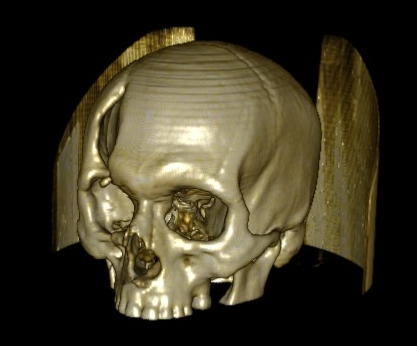
\includegraphics[scale=0.68]{brilhante_I}
\caption{Brilhante}
\label{fig:brilhante_I}
\end{figure}

\begin{figure}[!htb]
\centering 
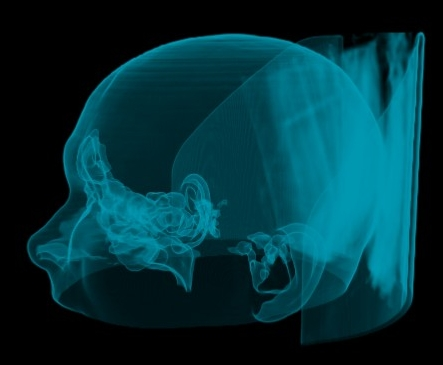
\includegraphics[scale=0.65]{vias_aereas_II}
\caption{Vias Aéreas II}
\label{fig:vias_aereas_II} 
\end{figure}

\begin{figure}[!htb]
\centering
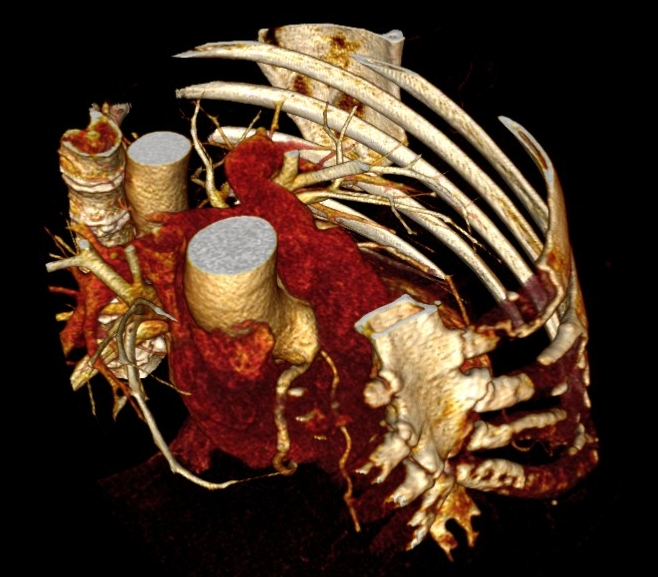
\includegraphics[scale=0.42]{contraste_medio}
\caption{Contraste Médio}
\label{fig:contraste_medio}
\end{figure}

\begin{figure}[!htb]
\centering
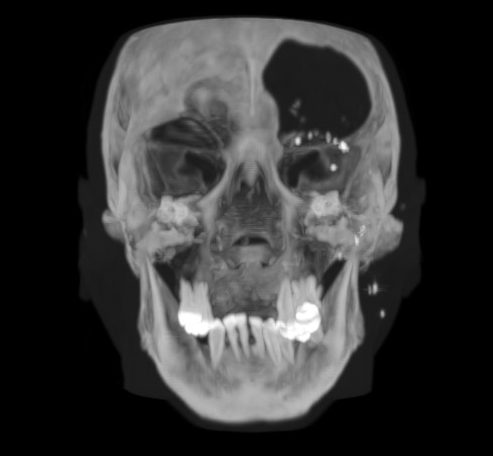
\includegraphics[scale=0.55]{MIP}
\caption{MIP}
\label{fig:MIP}
\end{figure}


\newpage


\section{Personalização de padrão}

Alguns padrões podem ser personalizados (ou customizados). Veja a figura
\ref{fig:customize_1}, que exibe um padrão e alguns controles gráficos de ajuste.
Com eles, é possível alterar a cor de uma dada estrutura e sua opacidade, determinando
como e se ela será exibida.

\begin{figure}[!htb]
\centering
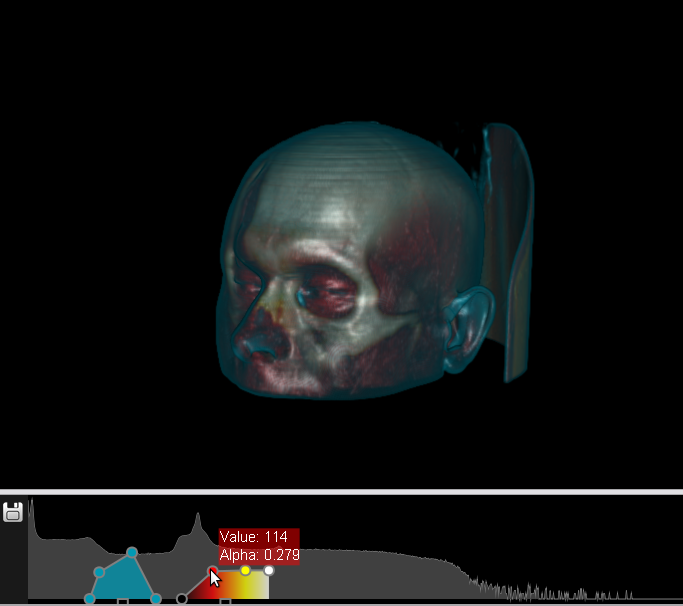
\includegraphics[scale=0.6]{customize_1}
\caption{Ajustes para o padrão de visualização Mole + Pele II}
\label{fig:customize_1}
\end{figure}


\newpage


Caso se deseje ocultar uma estrutura, é necessário utilizar o controle gráfico de ajuste mantendo
baixa a opacidade da região correspondente. No exemplo da figura \ref{fig:customize_1},
suponha que se pretende esconder a parte muscular, que aparece em vermelho. Para isso, basta
posicionar o ponteiro do mouse sobre o ponto em vermelho e, com o botão esquerdo pressionado,
\textbf{arrastar} o ponto para baixo, a fim de diminuir a opacidade (o que equivale a aumentar
a transparência). A figura \ref{fig:customize_2} ilustra o resultado.

Nota: O valor \textit{Alpha} indica a opacidade da cor, e o valor \textit{Value}, a
intensidade da cor no pixel.

\begin{figure}[!htb]
\centering
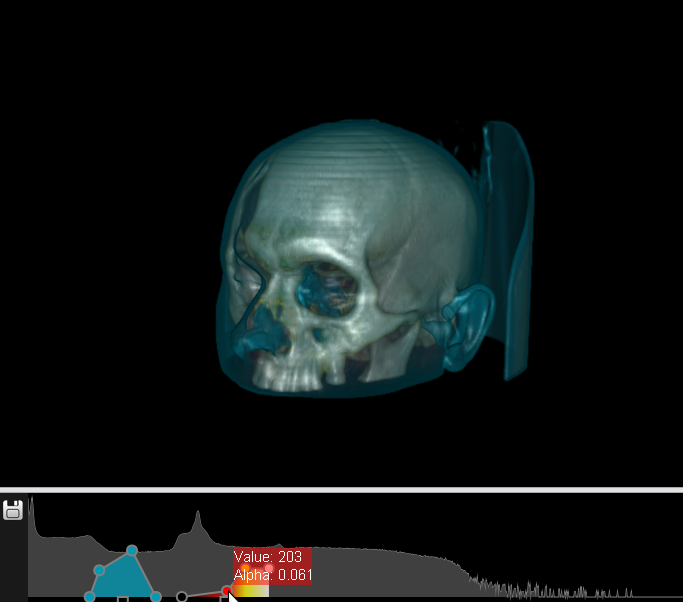
\includegraphics[scale=0.6]{customize_2}
\caption{Padrão de visualização Mole + Pele II alterado}
\label{fig:customize_2}
\end{figure}


\newpage


É possível remover ou adicionar pontos no controle gráfico de ajuste. Para a remoção, basta clicar
com o botão \textbf{direito} do mouse sobre o ponto. Para adicionar um novo ponto, clique com
o botão \textbf{esquerdo} sobre a linha do gráfico. Pode-se também salvar o padrão resultante,
clicando no atalho que a figura \ref{fig:save_preset} ilustra.

\begin{figure}[!htb]
\centering

\includegraphics[scale=0.6]{save_preset}
\caption{Atalho para salvar padrão}
\label{fig:save_preset}
\end{figure}
 
Ao salvar o padrão, o InVesalius exibe uma janela como a da figura \ref{fig:save_window_preset}.
Digite um nome para o padrão personalizado e clique em \textbf{OK}. O padrão salvo estará
disponível com os demais na próxima vez em que o software for aberto.

\begin{figure}[!htb]
\centering
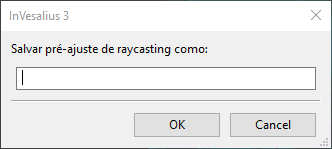
\includegraphics[scale=0.7]{save_window_preset_pt.png}
\caption{Janela para nomear e salvar um padrão}
\label{fig:save_window_preset}
\end{figure}

\section{Personalização de padrão com Brilho e Contraste}

É possível personalizar um padrão sem utilizar o controle gráfico de ajuste, apresentado na seção
anterior. Isso é feito por meio do controle de brilho e \textbf{Contraste} presente na barra de
ferramentas. Para ativar o controle, clique no atalho ilustrado pela figura
\ref{fig:tool_contrast_original_vol}.

\begin{figure}[!htb]
\centering

\includegraphics[scale=0.6]{tool_contrast_original}
\caption{Atalho para brilho e contraste}
\label{fig:tool_contrast_original_vol}
\end{figure}

Com o controle ativado, arrastando o mouse com o botão esquerdo pressionado
sobre a janela do volume, é possível alterar os valores de \textit{window width} e
\textit{window level}. O procedimento é o mesmo aplicado para as fatias 2D, visto
na seção \ref{sec:ww_wl}. Arrastando o mouse na direção horizontal, altera-se o valor de
\textit{window level}. Para a esquerda, diminui-se seu valor e, para a direita,
aumenta-se seu valor. Arrastando o mouse na direção vertical, altera-se o valor de
\textit{window width}. Para baixo, diminui-se seu valor e, para cima, aumenta-se seu
valor.

Com a manipulação desses valores, conseguem-se diferentes resultados de
visualização. Por exemplo, para adicionar tecido à visualização, \textbf{arraste} o
mouse diagonalmente, do canto inferior direito para o canto superior esquerdo da janela
de visualização. Para remover tecido da visualização, faça o contrário, ou seja,
\textbf{arraste} o mouse diagonalmente, do canto superior esquerdo para o canto inferior
direito. Veja a figura \ref{fig:raycasting_add}.

\begin{figure}[!htb]
  \centering
  \subfloat[Osso]{\label{fig:raycasting_add_1}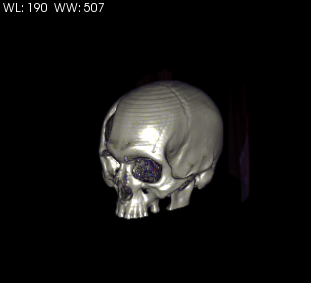
\includegraphics[width=0.33\textwidth]{raycasting_add_1}}                
  \hfill
  \subfloat[Músculo]{\label{fig:raycasting_add_2}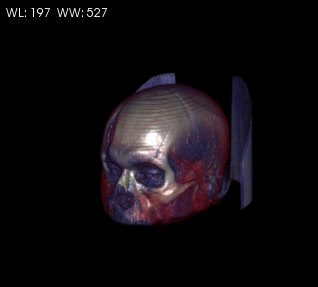
\includegraphics[width=0.333\textwidth]{raycasting_add_2}}	
  \hfill  
  \subfloat[Pele]{\label{fig:raycasting_add_3}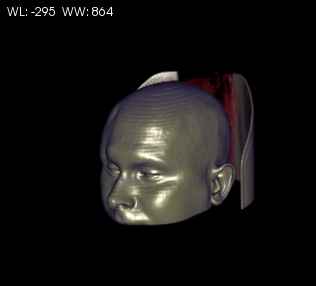
\includegraphics[width=0.332\textwidth]{raycasting_add_3}}
  \caption{Adição de tecido}
  \label{fig:raycasting_add}
\end{figure}

\newpage


\section{Corte}

Em visualização volumétrica, o corte é utilizado para visualizar uma região interna do volume.
O InVesalius dispõe de uma ferramenta para corte com base em um plano de referência. Com
um padrão de visualização selecionado, clique em \textbf{Ferramentas} e, em seguida, em
\textbf{Plano para corte} (figura \ref{fig:activate_cut_plane}).

\begin{figure}[!htb]
\centering
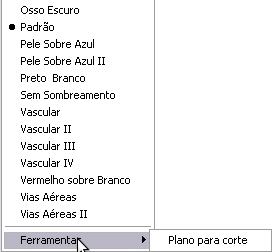
\includegraphics[scale=0.6]{activate_cut_plane_pt.png}
\caption{Ativando plano para corte}
\label{fig:activate_cut_plane}
\end{figure}

Uma representação do plano para corte é exibida junto ao volume. Para realizar o corte,
mantenha o botão \textbf{esquerdo} pressionado sobre o plano e \textbf{arraste} o mouse.
Para rotacionar o plano, mantenha o botão \textbf{esquerdo} pressionado sobre a sua borda
e movimente o mouse na direção desejada. Veja um exemplo na figura \ref{fig:cutted_image}.

\begin{figure}[!htb]
\centering
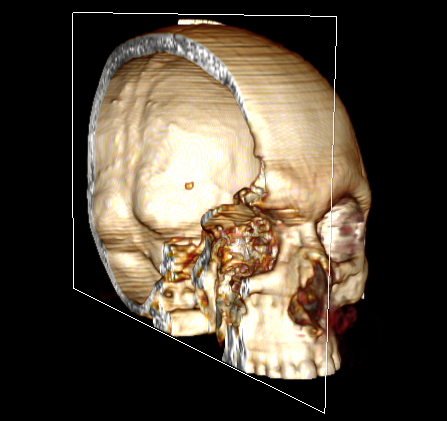
\includegraphics[scale=0.6]{cutted_image}
\caption{Imagem com plano de corte}
\label{fig:cutted_image}
\end{figure}

Para desativar o recurso de corte, clique novamente em \textbf{Ferramentas} e em
\textbf{Plano para corte} (figura \ref{fig:activate_cut_plane}).
